\documentclass[
  bibliography=totoc,     % Literatur im Inhaltsverzeichnis
  captions=tableheading,  % Tabellenüberschriften
  titlepage=firstiscover, % Titelseite ist Deckblatt
]{scrartcl}

% Paket float verbessern
\usepackage{scrhack}

% Warnung, falls nochmal kompiliert werden muss
\usepackage[aux]{rerunfilecheck}

% unverzichtbare Mathe-Befehle
\usepackage{amsmath}
% viele Mathe-Symbole
\usepackage{amssymb}
% Erweiterungen für amsmath
\usepackage{mathtools}

% Fonteinstellungen
\usepackage{fontspec}
% Latin Modern Fonts werden automatisch geladen
% Alternativ zum Beispiel:
%\setromanfont{Libertinus Serif}
%\setsansfont{Libertinus Sans}
%\setmonofont{Libertinus Mono}

% Wenn man andere Schriftarten gesetzt hat,
% sollte man das Seiten-Layout neu berechnen lassen
\recalctypearea{}

% deutsche Spracheinstellungen
\usepackage{polyglossia}
\setmainlanguage{german}


\usepackage[
  math-style=ISO,    % ┐
  bold-style=ISO,    % │
  sans-style=italic, % │ ISO-Standard folgen
  nabla=upright,     % │
  partial=upright,   % ┘
  warnings-off={           % ┐
    mathtools-colon,       % │ unnötige Warnungen ausschalten
    mathtools-overbracket, % │
  },                       % ┘
]{unicode-math}

% traditionelle Fonts für Mathematik
\setmathfont{Latin Modern Math}
% Alternativ zum Beispiel:
%\setmathfont{Libertinus Math}

\setmathfont{XITS Math}[range={scr, bfscr}]
\setmathfont{XITS Math}[range={cal, bfcal}, StylisticSet=1]

% Zahlen und Einheiten
\usepackage[
  locale=DE,                   % deutsche Einstellungen
  separate-uncertainty=true,   % immer Fehler mit \pm
  per-mode=symbol-or-fraction, % / in inline math, fraction in display math
]{siunitx}


% richtige Anführungszeichen
\usepackage[autostyle]{csquotes}

% schöne Brüche im Text
\usepackage{xfrac}

% Standardplatzierung für Floats einstellen
\usepackage{float}
\floatplacement{figure}{htbp}
\floatplacement{table}{htbp}

% Floats innerhalb einer Section halten
\usepackage[
  section, % Floats innerhalb der Section halten
  below,   % unterhalb der Section aber auf der selben Seite ist ok
]{placeins}

% Seite drehen für breite Tabellen: landscape Umgebung
\usepackage{pdflscape}

% Captions schöner machen.
\usepackage[
  labelfont=bf,        % Tabelle x: Abbildung y: ist jetzt fett
  font=small,          % Schrift etwas kleiner als Dokument
  width=0.9\textwidth, % maximale Breite einer Caption schmaler
]{caption}
% subfigure, subtable, subref
\usepackage{subcaption}

% Grafiken können eingebunden werden
\usepackage{graphicx}
% größere Variation von Dateinamen möglich
\usepackage{grffile}

% schöne Tabellen
\usepackage{booktabs}

% Verbesserungen am Schriftbild
\usepackage{microtype}

% Literaturverzeichnis
\usepackage[
  backend=biber,
]{biblatex}
% Quellendatenbank
\addbibresource{lit.bib}
\addbibresource{programme.bib}

% Hyperlinks im Dokument
\usepackage[
  unicode,        % Unicode in PDF-Attributen erlauben
  pdfusetitle,    % Titel, Autoren und Datum als PDF-Attribute
  pdfcreator={},  % ┐ PDF-Attribute säubern
  pdfproducer={}, % ┘
]{hyperref}
% erweiterte Bookmarks im PDF
\usepackage{bookmark}

% Trennung von Wörtern mit Strichen
\usepackage[shortcuts]{extdash}

\title{Versuch 101: Trägheitsmomente}
\author{Carolin Harkort \and Jacqueline Schlingmann}
\date{Durchführung: 27.10.2017, Abgabe:03.11.2017}

\begin{document}
%\maketitle

%\tableofcontents
%\newpage

\section{Zielsetzung}
\section{Theorie}

Als Trägheitsmoment wird der Widerstand eines Körpers gegen die Änderung seiner Rotation beschrieben,
welches abhängig von der Masse $M$ und dem Radius $r$ ist.
Die rotierenden Punktmasse besitzt ein Trägheitsmoment von $I = mr^2$.
Durch das Aufsummieren der einzelnen Trägheitsmomente wird das Gesamtträgheitsmoment berechnet.
\begin{align}
 I= \sum_{i = 0}^n r_i^2\cdot m_i
 \end{align}
 Entsprechend gilt für eine kontinuierliche Massenverteilung
 \begin{equation}
   \label{eqn:Trägheitsmoment}
   I = \int r^2\mathup{dm}
 \end{equation}

Zur Berechnung der Trägheitsmomente bekannter Symmetrien wurden folgenede Formeln verwendet:

\emph{Kugel}:

\begin{align}
  I_K = \frac{2}{5}mR^2
  \label{eqn:3}
\end{align}

\emph{Zylinder}:

\begin{align}
I_{Z} &= \frac{mR^2}{2} &
   I_{Zh} = m(\frac{R^2}{4} + \frac{h^2}{12})
   \label{eqn:4}
\end{align}

Wichtig zu beachten ist, dass dabei die Rotationsachse durch den Schwerpunkt des Körpers verläuft.
Ist dies nicht der Fall beschreibt der \textit{Satz von Steiner} die parallele Verschiebung
der Rotationsache, wobei $I_s$ als das Trägheitsmoment bezüglich der Schwerpunktsachse
und $a$ als der Abstand der Drehachse zur Schwerpunktsachse definiert ist.

\begin{equation}
  \label{eqn:Steiner}
  I = I_s +m\cdot a^2
\end{equation}

\subsection{Bestimmung der Trägheitsmomente}
Für das Drehmoment gilt
\begin{equation}
  \vec{M} = \vec{F} \times \vec{r}
  \label{eqn:6}
\end{equation}
In einem schwingungsfähigen System hängen Trägheitsmoment und Schwingungsdauer zusammen.
Dieser Zusammenhang wird durch

\begin{equation}
  T = 2\pi \sqrt{\frac{I}{D}}
  \label{eqn:7}
\end{equation}

beschrieben, wobei $I$ für das Trägheitsmoment des Körpers und $D$ für die
Winkelrichtgröße steht.
Für kleine Winkel lässt sich der Betrag des Drehmoments als

\begin{equation}
  M = D \cdot\varphi
  \label{eqn:8}
\end{equation}

mit dem Auslenkwenkel $\varphi$ darstellen.

\section{Durchführung}
\label{sec.Durchführung}

   \subsection{Bestimmung des Eigenträgheitsmoments}

   Zu Beginn wird eine Stange,
   die zuvor gewogen und ausgemessen wurde,
   auf der Apperatur festgeschraubt.
   Die Apperatur ist in Abbildung \ref{fig:1} zu sehen.
   Die Stange wird nun um zehn unterschiedliche Winkel $\varphi$ ausgelenkt.
   Zu jedem Winkel wird die wirkende Kraft mit einem Federkraftmesser bestimmt.
   Im Anschluss werden zwei Gewichte, die als symmetrisch angenommen werden,
   ausgemessen und gewogen.
   An der Stange befinden sich diese Gewichte jeweils zum selben Abstand von der Drehachse.
   Sie werden per Hand um einen bestimmten Winkel $\varphi$ ausgelenkt und losgelassen.
   Die Periodendauer $T$ der entstandenen Schwingung wird mittels einer Stopuhr bestimmt.
   Dies wird für zehn unterschiedliche Abstände von der Drehachse durchgeführt.

   \begin{figure}
    \centering
    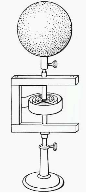
\includegraphics[scale=0.8]{V101_Aufbau.png}
    \caption{Aufbau der Apperatur am Beispiel einer Kugel}
    \label{fig:1}
   \end{figure}

   \subsection{Das Trägheitsmoment zwei unterschiedlicher Körper}

      Nun wird der Stab durch einen Zylinder ausgetauscht.
      Auch dieser wurde zuvor gewogen und ausgemessen.
      Der Körper besitzt eine Makierung, die als Nullpunkt verwendet wird
      um den Körper um einen
      gleichbleibenden Winkel $\varphi$ auszulenken.
      Es wird wieder die Periodendauer $T$ mittels einer Stoppuhr bestimmt.
      Der Vorgang wird fünfmal wiederholt und
      anschließend mit einer Kugel durchgeführt.

   \subsection{Trägheitsmoment einer Puppe}

      Die in 3.2 beschriebene Messung wird für eine Holzpuppe ebenfalls wiederhohlt.
      Dafür wird die Puppe gewogen und ausgemessen.
      Für die Ausmessung werden die Arme, der Rumpf, die Beine und der Kopf
      jeweils als Zylinder genährt.
      Die Breite jedes Körperteils ist fünf mal zu messen um einen Mittelwert
      des Radius für den Zylinder zu erhalten.
      Die Periodendauer $T$ wird für eine stehende Puppe mit ausgestreckten Armen bestimmt.
      Anschließend für diese Puppe in sitzender Position mit ausgestreckten Armen.

    \section{Auswertung}


   \subsection{Bestimmung der Winkelrichtgröße $D$ und des Eigenträgheitsmoments $I_D$}

   Der Kraftmesser hat zum Mittelpunkt einen Abstand von $\SI{20}{\centi\meter}$.
   Mit diesem Radius $r$ wird nun die Winkelrichtgröße $D$ bestimmt.
   Dafür werden die Formeln \ref{eqn:6} und \ref{eqn:8} verwendet.

   \begin{equation}
     D = (5{,}66 \pm 0{,}49) \cdot 10^{-4}\, \mathrm{Nm}
   \end{equation}
   Die Daten für diese Berechnung werden aus Tabelle \ref{tab:data2} entnommen.

   \begin{table}
     \centering
     \caption{Schwingungsdauern bei jeweiligen Abständen.}
     \label{tab:data2}
     \begin{tabular}{c c c c }
       \toprule $a \, \,  in \,\, m$ & $a^2 \,\, in \,\,  m^2$ & $T \,\, in \,\, s$ & $T^2 \,\, in  \,\, s^2$ \\
       \midrule
       0.03 & 0.0009 & 2.06 &  4.2436\\
       0.06 & 0.0036 & 2.29 &  5.2441\\
       0.09 & 0.0081 & 3.21 &  10.3041\\
       0.12 & 0.0144 & 4.16 &  17.3056\\
       0.15 & 0.0225 & 4.81 &  23.1361\\
       0.18 & 0.0324 & 5.41 &  29.2681\\
       0.21 & 0.0441 & 6.38 &  40.7044\\
       0.24 & 0.0579 & 7.16 &  51.2656\\
       0.27 & 0.0729 & 7.52 &  56.5504\\
       0.29 & 0.0841 & 8.49 &  72.0801\\
       \bottomrule
     \end{tabular}
   \end{table}
 Für die Berechnung des Eigenträgheitsmoments $I_D$ wird nun $T^2$ gegen $a^2$ aufgetragen.
 Dies ist in Abbildung \ref{fig:2} zu sehen.

   \begin{figure}
     \centering
     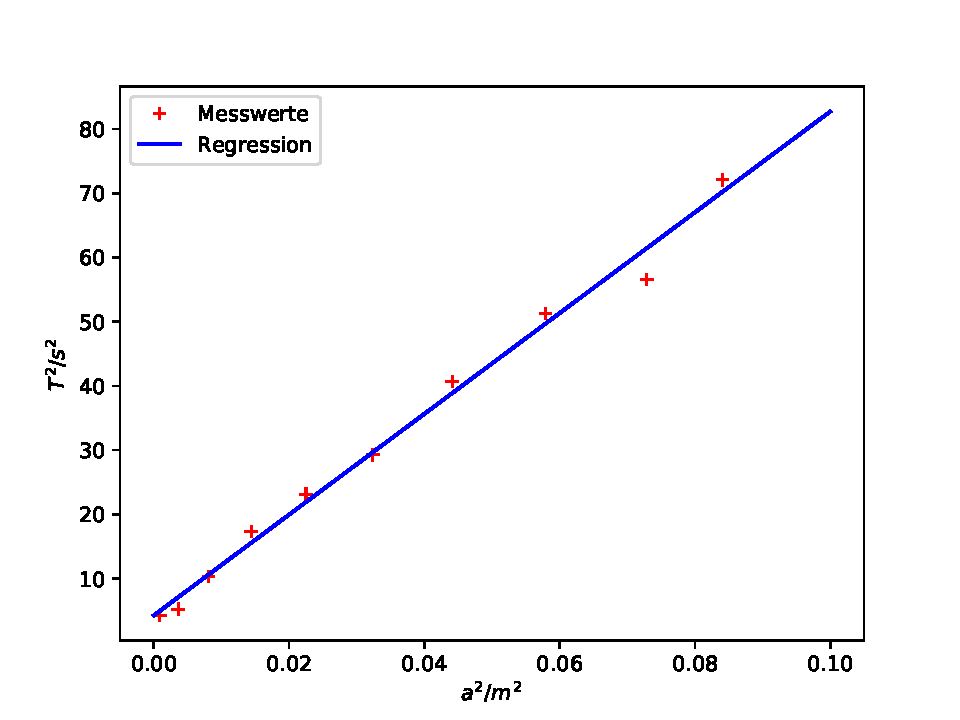
\includegraphics[width=\textwidth]{plot1.pdf}
     \caption{Die Quadrate der Schwingungsdauer gegenüber den Abstandsquadraten}
     \label{fig:2}
   \end{figure}

   Die lineare Regression wird mittels Python durchgeführt. Für die Gerade
   \begin{align}
     T^2 &= m * a^2 + n
   \end{align}
   ergeben sich die Steigung $m = (784 \pm 26) \frac{s^2}{m^2}$ und der y-Achsenabschnitt $n = (4.3 \pm 1.1) s^2$.

   Für die Berechnung des Eigenträgheitsmoments der Drillachse wird Formel\ref{eqn:4} und die Formel
   \begin{align}
   I_{Stange} &= \frac{1}{12} \cdot m_{Stange} \cdot H_{Stange}^2
   \end{align}
   für einen langen dünnen Stab verwendet. Mithilfe von
   \begin{align}
     I_D        &= I_{ges} - 2 \cdot I_{Z} - I_{Stange}\\
                &= \frac{b \cdot D_{dyn}}{4 \pi^2} - 2 \cdot I_{Z} - I_{Stange}\\
   \end{align}
   lässt sich das Eigenträgheitsmoment von
   \begin{equation}
     I_D = (-2.83 \pm 0.000)\cdot10^{-3} \symup{kg m^2}
   \end{equation}
bestimmen.

\subsection{Bestimmung der Trägheitsmomente zwei unterschiedlicher Körper}
\subsubsection{Trägheitsmoment eines Zylinders}
Zu Beginn der Messung werden von dem ausgewählten Zylinder die Radius, Höhe und Masse gemessen:
\begin{align}
  r_Z &= 0.04  \symup{m} \\ %Fehler?
  h_Z &= 0.14  \symup{m} \\
  m_Z &= 0.8995  \symup{kg}
\end{align}
Anhand dieser Werte wird das theoretische Trägheitsmoment bestimmt:
\begin{equation}
  I_{Zylinder,theo} = \frac{1}{2} m_Z \cdot r_Z^2 = 0.000720 \,\, \symup{kg m^2}
\end{equation}
%\begin{table}
  %\centering
  %\caption{Schwingungsdauer eines Zylinders}
  %\begin{tabular}{c c c c c c}
  %  \toprule $Messung$ & $1$ & $2$ & $3$ & $4$ & $5$ \\
  %  \midrule $Dauer [s]$ & 1.41 & 1.35 & 1.32 & 1.41 & 1.40\\
  %  \bottomrule
  %\end{tabular}
%\end{table}
Für die Schwingungsdauer ergibt sich dadurch %Bezug Tabelle
\begin{equation}
  T_{Zylinder} = (1.378 \pm 0.018) \symup{s}.
\end{equation}
und für das Trägheitsmoment des Zylinder
\begin{equation}
  I_{Zylinder,exp} = (0.0000198 \pm 0.000000)  \symup{kg m^2} %Fehler und Wert komisch, D=?
\end{equation}

\subsubsection{Trägheitsmoment einer Kugel}

Zunächst wird die Kugel ausgemessen und Gewogen.
\begin{align}
  r_K &= 0,695 \, \symup{m} \\
  m_K &= 0,8125 \, \symup{Kg}
\end{align}
Anhand dieser Werte kann nun das Trägheitsmoment $I_{Kugel, theo}$ bestimmt werden.
Dies geschieht mit Formel \ref{eqn:3}:
 \begin{equation}
   I_{Kugel,theo}= 0,0015698 \, \, \symup{kg \, m^2}
 \end{equation}
 Der experimentelle Wert für das Trägheitsmoment ermittelt sich aus Formel \ref{eqn:7}.
 Der Wert für die Schwingungsdauer $T$ wird mit Tabelle \ref{tab:schw} bestimmt.
Der Körper Wurde immer um einen Winkel von $ \frac{4\pi}{3}$ augelenkt.

 \begin{table}
   \centering
   \caption{Schwingungsdauer der Kugel}
   \label{tab:schw}
\begin{tabular}{cc}
  \toprule
  $Messung$ & $T \, \, in \, \, s$ \\
  \midrule
  1 & 1,63 \\
  2 & 1,55 \\
  3 & 1,55 \\
  4 & 1,53 \\
  5 & 1,58 \\
  \bottomrule
\end{tabular}
\end{table}
\begin{equation}
  T= (1{,}568 \pm 0{,}017) \, \mathrm{s}
\end{equation}
Der experimentelle Wert für das Trägheitsmoment lautet somit:
\begin{equation}
  I_{Kugel,exp}= (8{,}6566 \pm 0{,}1877) \cdot 10^{-3} \, \mathrm{Kg \, m^2} %bezug Fehlerrechnung
\end{equation}

\subsection{Bestimmung des Trägheitsmoments einer Puppe}

Für eine stehende Holzpuppe mit ausgestreckten Armen ergibt sich eine Schwingungsdauer von
\begin{equation}
  T= (1,446 \pm 0,051) \, \mathrm{s}
\end{equation}
und somit ein Trägheitsmoment ..., das nach Formel \ref{eqn:3} bestimmt wird.
Für diese Puppe mit ausgestreckten Armen und angewinkelten Beinen,
ergibt sich eine Schwingungsdauer
\begin{equation}
  T= (2,032 \pm 0,039) \, \mathrm{s}
\end{equation}
 und das Trägheitsmoment ...
Diese Holzpuppe hat ein Gewicht von
\begin{equation}
m= 0,03425 \, \mathrm{Kg}
\end{equation}
und wird als Zylinder genährt.
Dafür werden die Körperteile einzeln betrachtet.
Hierbei ist die Höhe bzw. die Länge  $h$ und der Radius $r$. \\

\emph{Kopf}:
\begin{align}
  h &= 0,071 \, \mathrm{m} & r &= (1,6725 \pm 0,051) \cdot 10^{-2} \, \mathrm{m}
\end{align}
\emph{Rumpf}:
\begin{align}
h &= 0,122 \, \mathrm{m} & r &= (2,292 \pm 0,406) \cdot 10^{-2} \, \mathrm{m}
\end{align}
\emph{Arm}:
\begin{align}
h &= 0,179 \, \mathrm{m} & r &= (0,871 \pm 0,051) \cdot 10^{-2} \, \mathrm{m}
\end{align}
\emph{Bein}:
\begin{align}
h &= 0,198 \, \mathrm{m} & r &= (0,932 \pm 0,145) \cdot 10^{-2} \, \mathrm{m}
\end{align}
Die Höhen und der Radius mit dem Fehler ergeben sich aus den gemessenen Werten,
die im Anhang zu finden sind.

Um das Trägheitsmoment bestimmen zu können müssen die Massen der einzelnen Körperteile bestimmt werden.
Dies geschieht mit der Formel
\begin{equation}
  m_{teil}= \frac{V_{teil}}{V_{ges}}\cdot m_{ges}
\end{equation}

Die dafür benötigten Volumen ergeben sich aus der Formel
\begin{equation}
  V_{Zylinder}= \pi \cdot r^2 \cdot h
\end{equation}
\begin{align}
  V_{Kopf} &= (0,6239366 \pm 0,0000038) \, \mathrm{m^3} \\
  V_{Rumf} &= (2,0134411 \pm 0,0000713) \, \mathrm{m^3} \\
  V_{Arme} &= (0,4266180 \pm 0,0000049) \, \mathrm{m^3} \\
  V_{Beine} &= (0,5403148 \pm 0,0000168) \, \mathrm{m^3} \\
  V_{Gesamt} &= (4,571233 \pm 0,000119) \, \mathrm{m^3}
\end{align}
Somit Ergeben sich nun die einzelnen Massen:
\begin{align}
  m_{Kopf} &= (4,67485 \pm 0,00012) \cdot 10^{-3} \, \mathrm{Kg}\\
  m_{Rumpf} &= (15,08572 \pm 0,00066)\cdot 10^{-3} \, \mathrm{Kg}\\
  m_{Arme} &= (3,19644) \pm 0,00009) \cdot 10^{-3} \, \mathrm{Kg}\\
  m_{Beine} &= (4,04831 \pm 0,00126) \cdot 10^{-3} \, \mathrm{Kg}
\end{align}
Die Massenangaben sind jeweils für beide Arme und Beine angegeben.
\subsection{Diskussion}
Die Messscheibe für die Winkelauslenkungen war nicht fest an der Apperatur befestigt.
Daher veschob sie sich leicht. Dies führt zu ungenauigkeiten bei der Auslenkung.
Hinzu kommen die Fehler, die beim Ablesen geschehen.
Bei der Holzpuppe kam es vorallem zu Messungenauikeiten,
da sie bei der Schwingung ihre Position nicht beibehalten konnte
und sich etwas verformt hat. Eine Messung mit angelegten Armen war nicht Möglich,
da diese fest in Waagerechter Stellung geklebt waren.

 \end{document}
